\documentclass[border=.1cm]{standalone}

\usepackage{tikz}
\usepackage{pgfplots}
\usepgflibrary{arrows}

\usepackage{siunitx}
\sisetup{
    detect-all = true,
    input-decimal-markers = {.},
    input-ignore = {,},
    inter-unit-product = \ensuremath{{}\cdot{}},
    multi-part-units = repeat,
    number-unit-product = \text{~},
    per-mode = fraction,
    separate-uncertainty = true,
}

\begin{document}

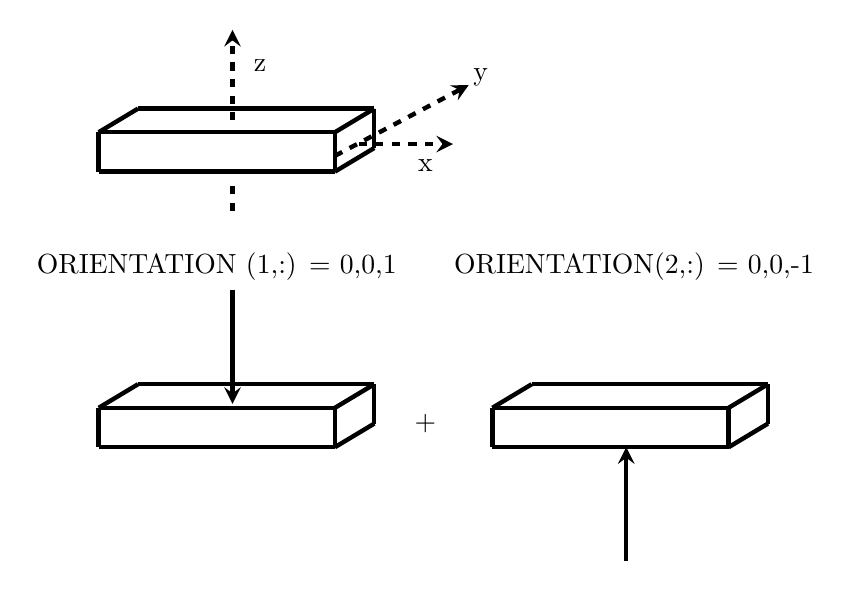
\begin{tikzpicture}

\draw [ultra thick]  (0,0) -- (0,.5); 
\draw [ultra thick]  (0,0) -- (3,0); 
\draw [ultra thick]  (3,0) -- (3,.5); 
\draw [ultra thick]  (0,.5) -- (3,.5); 
\draw [ultra thick]  (0,.5) -- (.5,.8); 
\draw [ultra thick]  (.5,.8) -- (3.5,.8); 
\draw [ultra thick]  (3,.5) -- (3.5,.8); 
\draw [ultra thick]  (3.5,.8) -- (3.5,.3);  
\draw [ultra thick]  (3,0) -- (3.5,.3); 
\draw [-stealth, ultra thick]  (1.7,2) -- (1.7,.55);  
\node at (1.5,2.3) {ORIENTATION (1,:) = 0,0,1}; 

\draw [ultra thick]  (5,0) -- (5,.5); 
\draw [ultra thick]  (5,0) -- (8,0); 
\draw [ultra thick]  (8,0) -- (8,.5); 
\draw [ultra thick]  (5,.5) -- (8,.5); 
\draw [ultra thick]  (5,.5) -- (5.5,.8); 
\draw [ultra thick]  (5.5,.8) -- (8.5,.8); 
\draw [ultra thick]  (8,.5) -- (8.5,.8); 
\draw [ultra thick]  (8.5,.8) -- (8.5,.3);  
\draw [ultra thick]  (8,0) -- (8.5,.3); 
\draw [-stealth, ultra thick]  (6.7,-1.45) -- (6.7,0);  
\node at (6.8,2.3) {ORIENTATION(2,:) = 0,0,-1};  

\node at (4.15,.3) {+};  
 
\draw [ultra thick]  (0,3.5) -- (0,4); 
\draw [ultra thick]  (0,3.5) -- (3,3.5); 
\draw [ultra thick]  (3,3.5) -- (3,4); 
\draw [ultra thick]  (0,4) -- (3,4); 
\draw [ultra thick]  (0,4) -- (.5,4.3); 
\draw [ultra thick]  (.5,4.3) -- (3.5,4.3); 
\draw [ultra thick]  (3,4) -- (3.5,4.3); 
\draw [ultra thick]  (3.5,4.3) -- (3.5,3.8);  
\draw [ultra thick]  (3,3.5) -- (3.5,3.8);  
\draw [-stealth, dashed, ultra thick]  (1.7,4.15) -- (1.7,5.3);     
\draw [ dashed, ultra thick]  (1.7,3) -- (1.7,3.4);     
\node at (2.05,4.85) {z};   
\draw [-stealth, dashed, ultra thick]  (3.3,3.85) -- (4.5,3.85);    
\node at (4.15,3.58) {x};   
\draw [-stealth,dashed,ultra thick]  (3,3.7) -- (4.7,4.6); 
\node at (4.85,4.7) {y};   







\end{tikzpicture}

\end{document}